\section{while语句}

\begin{frame}[fragile]\ft{\secname}
\begin{lstlisting}
while (condition)
  statement
\end{lstlisting}
\begin{lstlisting}
while (condition)
{
  statements
}
\end{lstlisting}
\end{frame}

\begin{frame}[fragile]\ft{\secname}
\begin{figure}
\centering
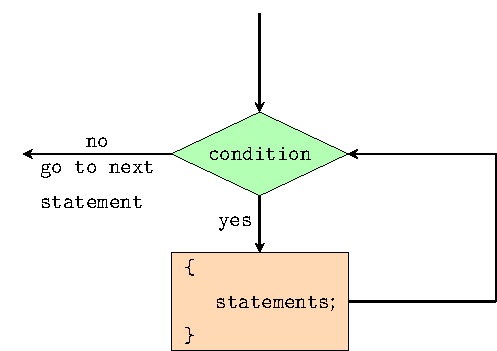
\includegraphics[width=4in]{ch06/images/while.pdf}
\end{figure}

\end{frame}

\begin{frame}[fragile]\ft{\secname:终止while循环}
构造一个while循环时,必须能改变判断表达式的值,并最终使其为假,否则循环永远不会终止。
\pause \vspace{.1in}

\begin{lstlisting}[language=c]
index = 1;
while (index < 5)
{
  printf("Good morning!\n");
}
\end{lstlisting} 
\pause \vspace{0.1in}

这段代码无法终止循环,因为在循环中不能改变index的值。
\end{frame}

\begin{frame}[fragile]\ft{\secname:终止while循环}
\begin{lstlisting}[language=c]
index = 1;
while (--index < 5)
{
  printf("Good morning!\n");
}
\end{lstlisting} 
\pause \vspace{0.1in}

虽然改变了index的值,但却朝着错误的方向,故仍无法退出循环。
\end{frame}

\begin{frame}[fragile]\ft{\secname:终止while循环}
\begin{lstlisting}[language=c]
index = 1;
while (++index < 5)
{
  printf("Good morning!\n");
}
\end{lstlisting} 
\pause \vspace{0.1in}

这段代码可以正常退出循环。
\end{frame}

\begin{frame}[fragile]\ft{\secname:何时终止循环}
只有在计算判断条件的值时才能决定是否终止循环。
\pause \vspace{.1in}

  \begin{minipage}{0.65\textwidth}
    \lstinputlisting[numbers=left]{ch06/code/when.c}    
  \end{minipage}~~~~\pause  
  \begin{minipage}{0.3\textwidth}
    \begin{lstlisting}
n = 5
Now n = 6
n = 6
Now n = 7
\end{lstlisting}
    
  \end{minipage}


\end{frame}

\begin{frame}[fragile]\ft{\secname:while:入口条件循环}
while循环是使用入口条件的有条件循环。 \pause \vspace{.1in}

\begin{lstlisting}
index = 10;
while (index++ < 5)
  printf("Have a fair day or better.\n");
\end{lstlisting}
\pause \vspace{.1in}

把第一行改为 \lstinline|index = 3;|,
就可以执行这个循环了。
\end{frame}

\begin{frame}[fragile]\ft{\secname:语法要点}
在使用while时,请确定循环体的范围。缩进是为了帮助读者而不是计算机。
\end{frame}

\begin{frame}[fragile]\ft{\secname:语法要点}
  \begin{minipage}{0.65\textwidth}
    \lstinputlisting[numbers=left]{ch06/code/while1.c}    
  \end{minipage} ~~~~\pause 
  \begin{minipage}{0.25\textwidth}
\begin{lstlisting}
n = 0
n = 0
n = 0
n = 0
... 
\end{lstlisting}    
  \end{minipage}
\end{frame}

\begin{frame}[fragile]\ft{\secname:语法要点}
while语句在语法上算作一条单独的语句,即使它使用了复合语句。 \vspace{.1in}

该语句从while开始,\vspace{.1in}
\begin{itemize}
  \item 若循环体只有一条语句,则到第一个分号结束;\\[.1in]
  \item 若循环体使用了复合语句,则到终结花括号结束。
\end{itemize}
\end{frame}

\begin{frame}[fragile]\ft{\secname:语法要点}
\lstinputlisting[language=c,frame=single,numbers=left]{ch06/code/while2.c}
\pause 
\begin{lstlisting}
n = 4
That's all this program does.
\end{lstlisting}
\end{frame}

\begin{frame}[fragile]\ft{\secname:语法要点}
  在C语言中,\red{单独的分号代表空语句(null statement)。}
\end{frame}

\begin{frame}[fragile]\ft{\secname:语法要点}
有些时候,程序员会有意地使用带空语句的while语句。
\vspace{.1in}

例如,假定你想要跳过输入直到第一个不为空或数字的字符,可以这样做。
\pause \vspace{.1in}

\begin{lstlisting}[language=c]
while(scanf("%d",&num)==1)
  ;
\end{lstlisting}\pause\vspace{.1in}

\red{为了清楚起见,请把分号单独置于while的下一行。}
\end{frame}

